% （本节重点见 §3 开头，由分片 E 负责）
%=====================================================================
%  分片 F：§3.6--§3.9（原文 PDF 第 54--65 页，止于第 65 页 §4 标题之前）
%  底本：translate/src/src_F.tex（sw.tex 第 3683--4322 行）
%  说明：本片从 §3 中部开始，故不写 keypoints；批注以“原文 PDF 第 N 页”定位，
%        公式括注原文 PDF 的连续编号（(97)--(108) 等），便于与原书对照。
%=====================================================================

\subsection{$SU(2)$ 理论模空间上的单值变换}

我们已讨论过模空间上存在单值变换的可能性，并指出：理解单值变换的结构或许有助于求解该理论，
即确定有效低能理论的精确非微扰预势。这等价于确定函数 $a_D(u)$ 与 $a(u)$。
本小节中，我们要找出模空间 ${\cal M}$ 上的奇点，并计算与之相应的单值变换。

% [Tutor Note: 原文笔误汇总（本分片）：“associalted”→“associated”（PDF 54）；
%  “close loop”→“closed loop”（PDF 54、61）；“elementary stat”→“elementary state”（PDF 56）；
%  “The the associated”→“The associated”（PDF 56）；“gauge theroy”→“gauge theory”、
%  “in terms our”→“in terms of our”（PDF 58）；“singuralites”→“singularities”（PDF 60）；
%  “Sine”→“Since”、“anyone”→“any one”（PDF 61）；“regrad”→“regard”、“Upto”→“up to”（PDF 62）；
%  “in terms complete”→“in terms of complete”（PDF 63）、“hypergeometirc”→“hypergeometric”（PDF 64）。
%  译文一律按正确拼写处理；所有公式照原文抄录，未作“修正”。]

\noindent\underline{大 $u$ 处的单值变换：}

在 $|a|$ 很大时，理论是渐近自由的，且 $u=\frac{1}{2}a^2$。在很好的近似下，预势由单圈公式
${\cal F}(a)=(i/2\pi)a^2\,{\rm ln}\, (a^2/\Lambda^2)$ 给出，由此得到
$$
a_D=\frac{\partial{\cal F}}{\partial a}=
\frac{2ia}{\pi}\,{\rm ln}\,(\frac{a}{\Lambda})+\frac{ia}{\pi}\,.
$$
若在 $u$ 平面上绕 $u=0$ 走一闭合回路，就有
${\rm ln}\,u \rightarrow {\rm ln}\,u+2\pi i$，${\rm ln}\,a \rightarrow {\rm ln}\,a+i\pi$，于是
$$
\begin{array}{rcl}
a_D & \rightarrow & - a_D + 2a \,,\\
a & \rightarrow & - a \,.
\end{array}
$$
这由单值矩阵
\begin{eqnarray}
M_{\infty}&=& PT^{-2}=\left(\begin{array}{cc}
-1 & 2 \\ 0 & -1 \end{array} \right )\,,
\label{mondone}
\end{eqnarray}
实现，它作用在 $(a_D, a)^T$ 上。这里 $P$ 是 $SL(2,{\rm Z})$ 中单位元的负矩阵，$T$ 的定义见 (\ref{ST})。
在该单值变换的作用下，BPS 态的磁量子数与电量子数按
$(n_m,n_e)\rightarrow (-n_m,-n_e-2n_m)$ 变化，因此质量公式保持不变。

% [Tutor Note: 式 (\ref{mondone})（原文编号 (97)，原文 PDF 第 54 页）有三处易错：
%  (1) 单值矩阵作用在列向量 $(a_D,a)^T$ 上，而电荷向量按 $(M^{-1})^T$ 变换（见原文 PDF 第 54 页
%      式 (97) 之前关于 $w=(n_m,n_e)\to wM^{-1}$ 的说明）；两者方向相反，写反会得到 $M_\infty^{-1}$。
%  (2) $M_\infty=PT^{-2}$ 中 $P=-I$ 是 $SL(2,{\rm Z})$ 的中心元，给出整体变号
%      $a\to -a,\ a_D\to -a_D$；$T^{-2}$ 给出 $a_D$ 的平移 $2a$。二者不可拆错。
%  (3) 这里的回路是绕 $u=0$ 的大回路，它与绕 $u=\infty$ 的回路同伦（$u$ 平面上两者只差一块可缩区域），
%      故记为 $M_\infty$；绕行方向取逆时针，若取顺时针则所有单值矩阵都取逆。]

\noindent\underline{有限 $u$ 处的单值变换：}

$u=\infty$ 处的单值变换意味着在 $u$ 平面别处还存在其他单值变换。若这些单值变换与 $M_\infty$ 对易，
则 $a^2$ 是一个良好的整体坐标。然而情况不可能如此，因为那样动能的正定性会遭到破坏。
要得到非阿贝尔的单值变换群，$u$ 平面上至少需要两个位于有限 $u$ 处的奇点，且绕它们有非平凡的单值变换。
这些奇点将由破缺了的离散对称性 $u\rightarrow -u$ 相联系。我们对额外奇点的数目作这一最小假设。
于是，同时包围这两个奇点的回路应当重现单值变换 $M_\infty$。

% [Tutor Note: 原文 PDF 第 55 页第一段。$M_\infty$ 把 $a\to -a$，故 $a^2$ 在 $M_\infty$ 下不变；
%  若其余单值变换都与 $M_\infty$ 对易，单值群便成为阿贝尔群，$a^2$ 才可能是整体坐标。但此时
%  $\tau=da_D/da$ 的虚部无法保持正定，动能项会变号——“非阿贝尔的单值群”与“度规正定”是同一件事
%  的两面；这正是原文断言“this cannot be the case”的物理内容，原文未展开。]

模空间上这些奇点的起源是什么？为得到威尔逊低能有效作用量，我们已经把理论中所有有质量态积掉。
有质量粒子的圈图于是在模空间上给出非平凡的度规。然而质量谱依赖于模 $u$，因而可能出现这样的情形：
对某些 $u$ 值，一些质量变为零。此时我们实际上是在积掉无质量态，从而在模空间上产生奇点。
奇点的性质，即与之相应的单值变换，取决于在奇点处变为无质量的粒子的性质。由于在有限 $u$
（非微扰区域）质量谱作为 $u$ 的函数并不已知，奇点无法直接找出。可行的做法是：假定某些一般态
在特定的 $u$ 值（例如 $u=1$ 与 $u=-1$）变为无质量，并求出相应的单值变换（例如 $M_1$ 与 $M_{-1}$）。
这些无质量态于是由条件 $M_1 M_{-1}=M_\infty$ 确定。

% [Tutor Note: 原文 PDF 第 55 页。严格说，威尔逊有效作用量是把有质量自由度积掉得到的；当某个质量
%  趋于零时，该自由度便不应再被积掉，有效作用量的解析结构在此失效，表现为模空间上的奇点。奇点的
%  单值变换由在奇点处变为无质量的粒子的量子数决定——这正是后文用 $(n_m,n_e)$ 标记 $M(n_m,n_e)$ 的原因。
%  术语 “integrate out” 译作“积掉”。]

朴素地看，人们或许会预期有质量的规范玻色子多重态在变为无质量时贡献奇点。经典上这发生在 $u=0$ 处，
而在量子理论中该点可能移到一个非零的 $u$。然而，正如 \cite{SW-I} 中所论证的，自旋为 1 的多重态
变为无质量并不能给出一致的图像。我们在此不再重复该论证。

理论中自旋 $\le 1/2$ 的其余有质量态只有磁单极与双子，由于自旋条件的限制，它们属于短的 $N=2$
多重态，因而是 BPS 态。这些态由超多重态描述。Seiberg 与 Witten 提出，奇点产生于其中某些非微扰态
变为无质量之时。现在的问题是要计算相应的单值变换。注意，磁单极与双子的超多重态无法以局域的方式
与理论的基本场耦合。然而，在关于对偶的小节中已经看到，可以转到理论的对偶描述，在其中某些对偶
规范场与磁单极或双子的耦合方式，恰好与通常规范场同单位电荷粒子的耦合方式相同。因此我们只需先
计算一个有质量带电超多重态变为无质量时的单值变换，然后利用对偶变换求出一般磁单极或双子的单值变换。
让我们考虑理论的这样一种对偶描述：其中某个磁单极或双子表现为基本态，并用一个字母——比如 $q$——
来标记该描述。在这个态无质量的点附近，所有有质量场都可被积掉，理论实质上是一个与超多重态耦合的
$U(1)$ 理论。若把该描述中标量场的真空期望值（vev）记为 $a(q)$，则单位电荷的 BPS 态在 $a(q)=0$ 时质量趋于零，这一条件在某个
$u=u_q$ 处得到满足。于是在该点附近，$a(q)$ 是良好的局部坐标，可展开为
$a(q)\approx c_q\,(u-u_q)$。此外，在该点附近，单圈 $U(1)$ $\beta$ 函数给出（见下一小节）：
$$
\tau (a(q))=-\frac{i}{\pi}\,{\rm ln}\,\frac{a(q)}{\Lambda}\,,
$$
由此得到
$$
a_D(q)=-\frac{i}{\pi}\,a(q)\,{\rm ln}\,\frac{a(q)}{\Lambda}+
\frac{i}{\pi} \,.
$$
沿围绕 $u_q$ 的闭合回路走一圈，使 $(u-u_q)\rightarrow e^{2\pi i} (u-u_q)$，便得到单值变换
\begin{equation}
\begin{array}{rcl}
a_D(q)& \rightarrow & a_D(q) + 2 a(q)\,,\\
a(q)  & \rightarrow & a(q)\,.
\end{array}
\label{mondq}
\end{equation}

% [Tutor Note: 式 (\ref{mondq})（原文编号 (98)，原文 PDF 第 56 页）。与式 (97) 对比：在大 $u$
%  （弱耦合）处 $a_D\to -a_D+2a$、$a\to -a$；在超多重态无质量点处 $a_D\to a_D+2a$、$a\to a$。
%  两者在 PSL(2,Z) 意义下只差一个整体 $P=-I$，即 $M_\infty$ 对应 $T^{-2}$。需注意 $-I\in\Gamma(2)$
%  （因为 $-1\equiv 1\pmod 2$），所以把 $M_\infty$ 写成 $PT^{-2}$ 并不影响“单值群由 $M_1,M_{-1}$
%  生成并等于 $\Gamma(2)$”这一结论；但若在模变换中忽略这个 $-I$，就会误把 $(a_D,a)$ 与
%  $(-a_D,-a)$ 当成同一个截面。]

现在计算一个 $(n_m,n_e)$ 双子变为无质量时的单值变换（若 $n_m$ 与 $n_e$ 互素，则该双子是稳定的
或临界稳定的）。第一步是找出理论的一种对偶描述，使该双子在其中表现为电荷为 $(0,1)$ 的基本态。
在一般的 $SL(2,{\rm Z})$ 变换下，我们得到一个 $\left(n_m(q),n_e(q)\right)$ 双子，满足
\begin{equation}
\left(\begin{array}{c}a_D(q)\\a(q)\end{array}\right)=
\left(\begin{array}{c}\alpha a_D + \beta a\\
                      \gamma a_D + \delta a \end{array}\right)\,,
\qquad
\left(\begin{array}{c}n_m(q)\\n_e(q)\end{array}\right)=
\left(\begin{array}{c}n_m\delta - n_e\gamma \\
                    -n_m\beta + n_e\alpha \end{array}\right)\,,
\label{asns}
\end{equation}
使得 $Z=n_m a_D + n_e a$ 保持不变。上式中 $\alpha\delta - \beta\gamma =1$。现在选取参数使
$n_m(q) =0, n_e(q)=1$。在这一选取下，$(a_D(q), a(q))$ 成为这样一组变量：该双子经由它们与
$SL(2,{\rm Z})$ 变换后的规范场耦合，其方式恰与单位电荷同通常规范场的耦合相同。特别地，当该双子
在模空间上某点变为无质量时，在这一描述中相应的单值变换由 (\ref{mondq}) 给出。把 (\ref{asns})
中的第一个方程反解，得到 $a_D=-\beta a(q) + n_e a_D(q)$ 与 $a=\alpha a(q) - n_m a_D (q)$。
于是容易求出单值变换对原有变量的作用为
\begin{equation}
\left(\begin{array}{c}a_D<本地路径>)\rightarrow 
\left(\begin{array}{cc}1+2n_e n_m & 2n_e^2\\
-2n_m^2 & 1-2n_e n_m \end{array}\right)\,
\left(\begin{array}{c}a_D<本地路径>)\,.
\label{mondn}
\end{equation}
记该单值矩阵为 $M(n_m,n_e)$，注意 ${\rm Tr}\,M(n_m,n_e)=2$。因此单值变换总属于
$SL(2,{\rm Z})$ 的抛物子群。

% [Tutor Note: 式 (\ref{asns})（原文编号 (99)，原文 PDF 第 56 页）。$SL(2,{\rm Z})$ 矩阵
%  $M=\left(\begin{smallmatrix}\alpha&\beta\\ \gamma&\delta\end{smallmatrix}\right)$ 作用在周期向量上为
%  $v\to Mv$；由 $Z=n_ma_D+n_ea$ 不变可知电荷向量按 $(M^{-1})^T$ 变换，即
%  $(n_m,n_e)\to(\delta n_m-\gamma n_e,\,-\beta n_m+\alpha n_e)$。原文第一分量写作 $n_m\delta-n_e\gamma$，
%  核对时极易把 $\gamma$ 与 $n_e$ 的配对弄错；第二分量同理。另注意 $\alpha\delta-\beta\gamma=1$
%  正是 $SL(2,{\rm Z})$ 的行列式条件。]

% [Tutor Note: 式 (\ref{mondn})（原文编号 (100)，原文 PDF 第 56 页）。${\rm Tr}\,M(n_m,n_e)=2$ 且
%  $M\ne\pm I$，故 $M$ 是 $SL(2,{\rm Z})$ 中的抛物型元素，必与 $T$ 共轭；这是“只需两个奇点就能生成
%  整个单值群”的群论根据。矩阵元 $2n_e^2$、$-2n_m^2$ 中的因子 2 来自单圈 $\beta$ 函数（见下一小节），
%  不是笔误。]

现在计算 $u=\pm 1$ 处的单值变换。假定一个 $(m,n)$ 双子（dyon）在 $u=1$ 处变为无质量，一个
$(m',n')$ 双子（dyon）在 $u=-1$ 处变为无质量。于是相应的单值变换应满足
\begin{equation}
M_1(m,n)\,M_{-1}(m',n') = M (\infty)\,.
\label{mondeq}
\end{equation}
利用 (\ref{mondone}) 与 (\ref{mondn})，上式可以写成
$$
\left ( \begin{array}{cccc} 1 + 2mn & 2n^{2} \\ -2m^{2} & 1-2mn
\end{array} \right ) =
\left( \begin{array}{cccc} -1 & 2 \\ 0 & -1 \end{array} \right )
\left ( \begin{array}{cccc} 1-2m'n' & -2n'^{2} \\
2m'^{2} & 1 + 2m'n' \end{array} \right )\,,
$$
由此得到方程
$$
\begin{array}{rcl}
1 + mn &=& m'n' + 2m'^{2} \,,\\
m^{2} &=& m'^{2} \,,\\
n^{2} &=& n'^{2} + 1 + 2m'n'\,, \\
1 - mn &=& -m'n'\,.
\end{array}
$$
这些方程给出 $m=\pm 1$ 与 $m'=\pm 1$。对每一种 $(m,m')$ 组合，都可容易地确定 $n'$ 作为 $n$ 的函数，
得到如下可能的解集
$$
\begin{array}{cccccccc}
(m,n): &(1,n)&,&(-1, n)&,&(-1, n)&,&(1, n)\,,\\
(m',n'): &(1, n-1)&,&(1, -n-1)&,&(-1, n+1)&,&(-1, -n+1)\,. 
\end{array}
$$
似乎不存在把 $M_{\infty}$ 分解为多于两个这种抛物型 $M(m,n)$ 之乘积的解。此外注意，该解只允许
单位磁荷的双子对单值变换有贡献。这与半经典结果一致：只有这些双子是稳定的。

% [Tutor Note: 原文 PDF 第 56 页式 (101) 之后的解集。由矩阵等式得到四个方程，其中 $m^2=m'^2$
%  只给出 $m=\pm m'$，还需与 $1+mn=m'n'+2m'^2$、$1-mn=-m'n'$ 联立才能定出 $m,m'=\pm 1$。
%  表中四列依次对应 $(m,m')=(1,1),(1,-1),(-1,-1),(-1,1)$，最简单的解 $m=m'=1,n=0,n'=-1$
%  是第一列。另注意矩阵等式的左端是 $M_1$、右端是 $M_\infty M_{-1}^{-1}$，与式 (101) 的乘积次序
%  $M_1M_{-1}=M_\infty$ 一致；若把次序写反，所得方程会变成另一组。]

让我们再作一项一致性检验：一般说来，在单值变换的作用下，双子的量子数会改变。然而我们预期，
那个变为无质量、并且是奇点之源的特殊双子，应当在单值变换下保持不变（因为正是它的性质决定了
单值矩阵）。这可以容易地验证。本征值方程
\begin{equation}
(q_m, q_{e}) \left( \begin{array}{cc}
1+2mn & 2n^{2} \\ -2m^{2} & 1-2mn \end{array} \right ) =
(q_m, q_{e})\,,
\label{mon-inv}
\end{equation}
给出 $nq_m-mq_e=0$，前提是 $m$ 与 $n$ 不同时为零。显然，$q_m=m, q_n=n$ 是该方程的一个解。
若只限于稳定双子，则这是唯一的解。因此，已知单值变换，便能找出产生它的双子。

% [Tutor Note: 式 (\ref{mon-inv})（原文编号 (102)，原文 PDF 第 57 页）之后。原文 “Clearly,
%  $q_m=m, q_n=n$ is a solution” 中 $q_n$ 应为 $q_e$（本征向量按 $(q_m,q_e)$ 排列，见式 (102) 左端）；
%  这是原文笔误，公式本身无误。该本征值方程只定出 $(q_m,q_e)$ 的方向：$nq_m-mq_e=0$ 的通解为
%  $(q_m,q_e)\propto(m,n)$；对稳定双子取最小整数倍，才得到唯一的 $(m,n)$。]

方程 (\ref{mondeq}) 最简单的解对应 $m=m'=1, n=0, n'=-1$。此时单值矩阵为
\begin{equation}
M_1=\left(\begin{array}{cc}1&0\\-2&1\end{array}\right),\qquad
M_{-1}=\left(\begin{array}{cc}-1&2\\-2&3\end{array}\right)\,.
\label{mondothers}
\end{equation}
与 (\ref{mon-inv}) 比较可知：$M_1$ 源于一个磁单极在 $u=1$ 处变为无质量；$M_{-1}$ 则源于一个
$(1,-1)$ 双子（dyon）在 $u=-1$ 处变为无质量。在磁单极变为无质量的点处有 $a_D=0$；在 $(1,-1)$
双子变为无质量的点处有 $a-a_D=0$——由 $Z=n_m a_D + n_e a$ 即可看出。注意，无穷远处的单值变换
$M_\infty$ 把电荷平移 $2$ 个单位。因此，在发生凝聚的奇点处，电荷实际上只在模 $2$ 意义下定义。
我们可以用 $M^{n}_{\infty}$ 对基本群的表示作共轭。

% [Tutor Note: 原文 PDF 第 57 页末。$M_\infty$ 对电荷的作用是
%  $(n_m,n_e)\to(-n_m,-n_e-2n_m)$（见第 54 页），故在磁荷固定的扇区里，电荷只在模 $2n_m$
%  的意义下定义；对 $n_m=1$ 就是模 2。用 $M_\infty^n$ 共轭只改变基本群表示的基底（即单值矩阵的
%  起点），不改变物理；但它会改变“哪个双子表现为基本态”的标记，后文取 $M_1,M_{-1}$ 的表示时
%  已固定了这一基底。]

\subsection{$U(1)\; \beta$ 函数}

在上一小节构造单值变换时，我们用到了 $\beta$ 函数（针对与超多重态耦合的 $U(1)$ 理论）。下面更细致地
考察这一点。若理论中有电荷为 $Q_{f}$ 的 Weyl 费米子与电荷为 $Q_{s}$ 的复标量，则它们对
$U(1) \beta$ 函数的贡献为
$$
\beta(g)\equiv\mu \frac{d}{d \mu}g = \frac{g^{3}}{16\pi^{2}} \,
\left( \sum_{f} \; \frac{2}{3} Q^{2}_{f} +
\sum_{s} \; \frac{1}{3} Q^{2}_{s} \right )\,.
$$
若把 $g^3$ 的系数记为 $b$，并定义 $\alpha= g^2/4\pi$，则上式可改写成
$$
\mu \frac{d}{d\mu} \left( \frac{1}{\alpha} \right) = - 8\pi b\,.
$$
考虑一个超多重态，它是 $N = 2$ 的自旋 $\leq 1/2$ 的约化多重态。用 $N=1$ 语言，它由手征超场
$M,\widetilde M$ 描述，包含两个 Weyl 费米子与两个复标量，它们都带相同的电荷 $Q$。于是得到
$$
b = \frac{1}{16\pi^{2}} \; Q^{2} \left(2 \cdot \frac{2}{3} +
2 \cdot \frac{1}{3} \right) = \frac{1}{8\pi^{2}}\; Q^{2}\,.
$$
现在记住，我们已利用反常通过费米子的手征转动把 $\theta$ 参数取为零。结果有 $\tau=i/\alpha$，从而
$$
\mu \frac{d\tau}{d\mu} = - \frac{i}{\pi} Q^{2}\,.
$$
把 $\mu$ 认作理论的自然能标，即 $a$，并令 $Q=1$，得到
$$
\tau \simeq - \frac{i}{\pi}\,{\rm ln}\,\frac{a}{\Lambda}\,.
$$
这正是确定有限 $u$ 处单值变换时所用的表达式。若关心磁单极多重态的贡献，则可用对偶变量重复上述
计算，结果成为 $\tau_D\simeq -(i/\pi)\, {\rm ln}\,(a_D/\Lambda)$。

% [Tutor Note: 原文 PDF 第 57--58 页 $\beta$ 函数一节。这里 $b$ 定义为 $\beta(g)=b\,g^3$ 中 $g^3$
%  的系数（已含 $1/16\pi^2$），故 $\mu\,d(1/\alpha)/d\mu=-8\pi b$ 中的因子是 $8\pi$ 而不是 $2\pi$；
%  由 $\alpha=g^2/4\pi$ 可直接验证：$d(1/\alpha)/d\ln\mu=-(8\pi/g^3)\beta(g)$。系数 $2/3$ 与 $1/3$
%  分别是外尔费米子与复标量的标准单圈贡献，最易抄错。]

% [Tutor Note: 原文 PDF 第 58 页。一个超多重态含两个外尔费米子、两个复标量，故
%  $2\cdot\frac{2}{3}+2\cdot\frac{1}{3}=2$，得 $b=Q^2/8\pi^2$。这里每个外尔费米子贡献
%  $2Q_f^2/3$、每个复标量贡献 $Q_s^2/3$（均以 $g^3/16\pi^2$ 为单位）；$b>0$ 表明该 $U(1)$
%  在紫外并不渐近自由，而是红外自由（紫外出现朗道极点）。]

% [Tutor Note: 原文 PDF 第 58 页。用费米子的手征转动把 $\theta$ 参数转掉，前提是只关心 $\theta=0$
%  的真空；一般情形 $\tau=\theta/2\pi+i/\alpha$，$\mu\,d\tau/d\mu=-iQ^2/\pi$ 只对虚部成立。此处
%  “反常”指 $U(1)_R$ 的手征反常，它使 $\theta$ 的移动可完全转移到费米子相位上。对磁单极多重态，
%  把上述计算整体搬到对偶变量即得 $\tau_D\simeq-(i/\pi)\ln(a_D/\Lambda)$；注意 $\tau_D$ 与 $\tau$
%  不是同一个函数，在强耦合区不能混用。]

\subsection{磁单极凝聚与禁闭}

本小节中，我们说明 $N = 1$ 规范理论中的禁闭如何能在我们的宏观 $N=2$ 理论框架内得到理解。
$N = 2$ 的矢量超场 ${\cal A}$ 在 $N=1$ 形式下可分解为一个矢量超场 $W_{\alpha}$ 与一个手征超场
$\Phi$。要把 $N = 2$ 破缺到 $N = 1$，可以在作用量中加一项超势 $W=m\; {\rm Tr}\Phi^2$。这给
$\Phi$ 多重态一个裸质量，因此低能理论是一个纯阿贝尔规范理论。该低能理论具有 ${\bf Z}_{4}$ 手征
对称性，并被认为有质量间隙，同时伴随禁闭以及 ${\bf Z}_4$ 到 ${\bf Z}_2$ 的自发破缺。
Seiberg 与 Witten 基于 $N=2$ 的图像给出了这一现象的宏观描述，下面将加以说明。

% [Tutor Note: 原文 PDF 第 58 页（本小节开头）有两处笔误：“gauge theroy” 应为 “gauge theory”，
%  “in terms our” 应为 “in terms of our”。另注意：加 $W=m\,{\rm Tr}\Phi^2$ 使 $N=2$ 破缺到 $N=1$；
%  低能纯阿贝尔理论被认为有质量间隙，并自发破缺 $\mathbf{Z}_4\to\mathbf{Z}_2$，这是 $N=1$
%  规范理论禁闭的宏观图像，下文用磁单极凝聚来“实现”它。]

在 $N=2$ 理论中，半经典极限下的无质量谱只包含阿贝尔矢量多重态 ${\cal A}$。让我们分析开启
质量 $m$ 对标量多重态 $\Phi$ 的效果。在低能理论中，${\rm Tr}\,\Phi^2$ 由手征超场 $U$ 表示。
其标量分量为 $u =\langle{\rm Tr}\phi^2\rangle$，它是模空间上的全纯函数。对小的 $m$，可以直接在
低能拉格朗日量中加上 $W_{eff} = mU$。这大概会消除真空简并，并给标量多重态一个质量。要使阿贝尔
规范场也有质量（从而理论具有质量间隙），我们需要：(i) 额外的轻规范场，给出强耦合的非阿贝尔理论；
或者 (ii) 轻的带电场，给出希格斯机制。因此，无论哪种情形，在 ${\cal M}$ 上某处都必须出现额外的
无质量态。如前所述，不可能得到额外的轻规范场。因此我们考虑方案 (ii)，其中轻的带电场是磁单极或
双子。在无质量磁单极所在的点附近，我们转到理论的对偶描述，并用 $N=1$ 的手征超场
$M, \widetilde M$ 描述磁单极超多重态。在这一对偶描述中，完整的 $N=1$ 超势成为
$$
\hat{W} = \sqrt{2} A_{D} M \widetilde M + m \; U(A_{D})\,.
$$
低能真空结构容易分析。真空对应
$$
d \hat{W} = 0\,,
$$
的解，并满足 $|M| = |\widetilde M|$，从而使 $D$ 项为零。当 $m=0$ 时，$M=\widetilde M =0$ 而
$a_{D}$ 任意。于是我们回到 $N=2$ 的模空间。若 $m \not= 0$，则
\begin{eqnarray}
&{\displaystyle
\sqrt{2} M \widetilde M + m \; \frac{du}{dA_{D}} = 0} &\,,\nonumber \\
& a_{D}M = a_{D}\widetilde M = 0 &\,.\nonumber 
\end{eqnarray}
假定 $du/da_{D} \not= 0$，便得到 $M, \widetilde M\not= 0$，从而 $a_D=0$ 且
$M=\widetilde M=(-m u'(0)/\sqrt{2})^{1/2}$。由于 $M$ 带电，其真空期望值通过希格斯机制为规范场
产生质量。于是，通过简单的分析，我们重现了微观理论所预期的质量间隙。要理解电荷禁闭，注意：
由于超多重态 $M\widetilde M$ 描述磁单极，我们有一个磁希格斯机制。因此 $M\ne 0$ 意味着无质量的
磁单极在真空中凝聚。这通过（对偶的，即磁的）迈斯纳效应导致电荷的禁闭。

% [Tutor Note: 原文 PDF 第 59 页。由 $\hat W=\sqrt2 A_DM\widetilde M+mU(A_D)$ 得
%  $\partial\hat W/\partial M=\sqrt2 A_D\widetilde M$、
%  $\partial\hat W/\partial\widetilde M=\sqrt2 A_DM$、
%  $\partial\hat W/\partial A_D=\sqrt2 M\widetilde M+m\,du/dA_D$，三式令零即得文中两行方程
%  （第二行把两个方程合并书写，原文用小写 $a_D$ 指其标量分量）。$M=\widetilde M=(-m u'(0)/\sqrt2)^{1/2}$
%  中的 $u'(0)$ 指 $du/da_D$ 在 $a_D=0$ 处的值；原文未讨论根号下为负（此时取纯虚相位）的约定。这一相位只影响凝聚体的相位，$M\ne0$（从而磁希格斯机制成立）的结论不变。]

\subsection{模型的解}

本小节中，我们将把 $N=2$ 理论的模空间等同于亏格为 1 的黎曼面的模空间，并利用这一等同来计算
$a_D(u)$ 与 $a(u)$。

让我们先总结一下关于模空间结构已得到的认识：模空间 ${\cal M}$ 是 $u$ 平面，其奇点为
$1, -1, \infty$，另有 ${\bf Z}_{2}$ 对称性，作用为 $u \rightarrow -u$（图 3）。在这个带孔的平面上
存在一个平坦的 $SL(2,{\bf Z})$ 丛 $V$，它以 $(a_D, a)^T$ 为一个截面。该丛在奇点周围有如下单值
变换
\begin{equation}
M_{1} = \left( \begin{array}{cc}
1 & 0 \\ -2 & 1 \end{array} \right )\,, \quad
M_{-1} = \left( \begin{array}{cc}
-1 & 2 \\ -2 & 3 \end{array} \right )\,, \quad
M_{\infty} = \left( \begin{array}{cc}
-1 & 2 \\ 0 & -1 \end{array} \right )\,,
\label{mondall}
\end{equation}

\begin{figure}[htbp]
  \centering
  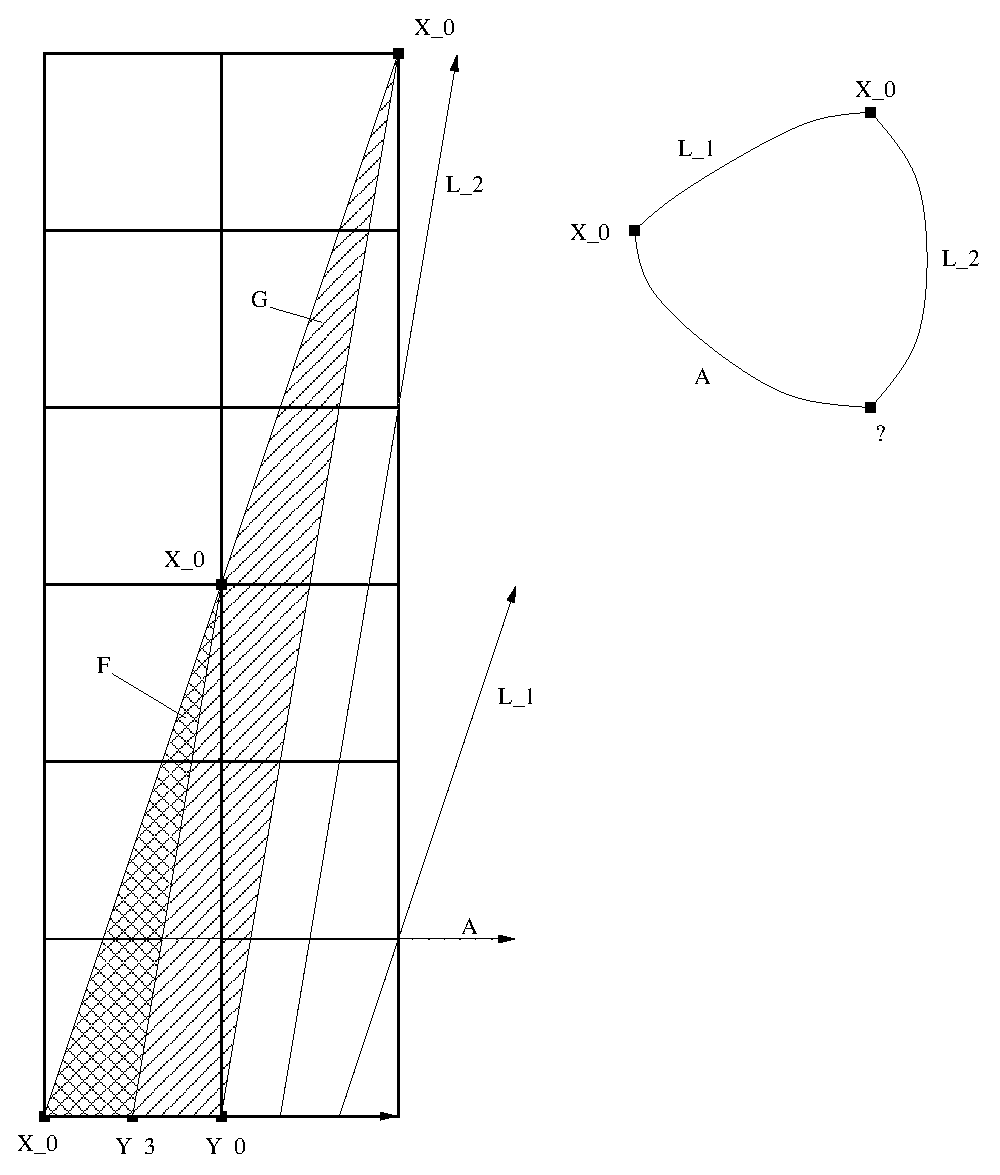
\includegraphics[width=0.45\textwidth]{figures/fig3.pdf}
  \caption{$u$ 平面上的奇点与单值变换。奇点位于 $u=-1,\,1,\,\infty$；绕 $u=-1$、$u=1$ 的回路分别给出
           单值矩阵 $M_{-1}$、$M_{1}$，绕无穷远的回路给出 $M_\infty=M_1M_{-1}$。原文仅标 “Figure 3”
           （原文 PDF 第 60 页），无说明性图注。}
  \label{fig:3}
\end{figure}

% [Tutor Note: 图 3（原文 PDF 第 60 页）与原文 PDF 第 59--60 页的丛语言。$u$ 平面去掉三个奇点后，
%  周期向量 $(a_D,a)^T$ 是平坦 $SL(2,{\rm Z})$ 丛 $V$ 的全纯截面；绕 $u=-1$、$u=1$、$u=\infty$ 的
%  回路分别给出 $M_{-1},M_1,M_\infty$，且按回路的复合次序 $M_\infty=M_1M_{-1}$（先绕 $u=-1$，
%  再绕 $u=1$，合成回路等效于绕无穷远）。把乘积次序写反会得到 $M_\infty^{-1}$。]

更确切地说，$(a_D(u), a(u))$ 构成丛 $V\otimes {\bf C}$ 的全纯截面，并具有如下渐近行为
\begin{eqnarray}
u\approx \infty\,:&\qquad& \left\{\, \begin{array}{l}
a \cong \sqrt{2u}\,  \\
a_D \approx i\;\frac{\sqrt{2u}}{\pi}\;{\rm ln}\; u
\end{array} \right. \,, \nonumber\\
u=1\,:&\qquad& \left\{\, \begin{array}{l}
a_D \approx \,c_0 (u-1) \\
a \approx a_0 + \frac{i}{\pi} \; a_{D}{\rm ln}\; a_{D}
\end{array} \right. \,.\nonumber
\end{eqnarray}
其中 $a_0$ 与 $c_0$ 为常数。对 $u=-1$，行为与 $u=1$ 类似，只需把 $a_D$ 换为 $a-a_D$。
模空间上的度规为 $ds^2={\rm Im}(\tau)\,|da|^2$，其中
\begin{equation}
\tau =\frac{da_D/du}{da / du}\,.
\label{tau-metric}
\end{equation}
为保证动能的正定性，${\rm Im}(\tau)$ 应当是正定的。这些单值变换生成子群 $\Gamma(2)$，它包含在 $SL(2,{\rm Z})$ 中；事实上，带奇点的 $u$ 平面就是上半平面 $H$ 对 $\Gamma(2)$ 的商。该商有三个尖点，
对应三个奇点。

% [Tutor Note: 原文 PDF 第 60 页未编号的渐近行为公式。弱耦合下 $u=\frac12a^2$（原文第 54 页），
%  故 $a\cong\sqrt{2u}$；而 $a_D\approx i\frac{\sqrt{2u}}{\pi}\ln u$ 中的 $i$ 与 $\pi$ 来自单圈预势
%  （见第 54 页 $\partial{\cal F}/\partial a$ 一式）。注意此式是对 $u$ 取对数，而不是对 $a$ 取对数，
%  二者相差 $\ln a^2=2\ln a$ 的常数项。在 $u=1$ 附近，$a_D\approx c_0(u-1)$ 是“磁单极无质量”的标志，
%  而 $a\approx a_0+\frac{i}{\pi}a_D\ln a_D$ 表明此时 $a_D$ 才是好坐标、$a$ 是坏坐标；$u=-1$ 处
%  作替换 $a_D\to a-a_D$。]

% [Tutor Note: 式 (\ref{tau-metric})（原文编号 (105)，原文 PDF 第 60 页）。$\tau=da_D/da$ 在 $u$
%  坐标下写成 $(da_D/du)/(da/du)$；弱耦合区 $\tau=\theta/2\pi+4\pi i/g^2$，故
%  ${\rm Im}\,\tau=4\pi/g^2>0$ 正是动能项正定。$S$ 对偶 $\tau\to-1/\tau$ 伴随
%  $(a_D,a)\to(a,-a_D)$ 的 $SL(2,{\rm Z})$ 作用，即“电—磁”互换；不要把 $a_D$ 与 $a$ 误当成纯虚、
%  纯实的量，它们一般是复的，只有 $\tau$ 的虚部才有正定意义（原文此处对“虚实变换”未加说明）。]

空间 $H/\Gamma(2)$（即 $u$ 平面）也参数化一族曲线 $E_u$，它们由方程
\begin{equation}
y^2 = (x-1)(x+1)(x-u)\,, 
\label{cubic}
\end{equation}
描述，其中 $x$ 是复变量。首先注意，该方程在变换
$$
w:\{u\rightarrow -u\,,x\rightarrow -x\,,y\rightarrow \pm iy \}\,,
$$
下不变；这些变换生成 ${\bf Z}_{4}$ 对称性，其中只有 ${\bf Z}_{2}$ 子群作用在 $u$ 上。
这与 ${\cal M}$ 上的对称性结构相同。现在来描述上述方程所代表的曲线。曲线基本上就是 $x$ 空间，
其拓扑由“$y$ 是单值函数”这一要求决定。由于方程对 $y$ 是二次的，若在 $x$ 空间沿绕 $y$ 的任意
一个零点的闭合回路走一圈，就有 $y\rightarrow -y$。对包含全部零点的回路也同样如此；等价地说，
绕 $x=\infty$ 的回路也如此（这是因为零点数为奇数）。因此，要使 $y$ 成为单值函数，$x$ 空间应当
是复平面 ${\bf C}$（再补上无穷远点）的双重覆叠。此外，该空间应在 $x=-1,1,u,\infty$ 处有四个
分支点，它们两两由两条割线相连（图 4）。为明确起见，取一条从 $-1$ 到 $1$ 的分支割线，另一条
从 $u$ 到 $\infty$。两张叶沿这些割线相接，使得穿过割线时从一张叶走到另一张叶。$y$ 正是在这个
空间上单值。

% [Tutor Note: 式 (\ref{cubic})（原文编号 (106)，原文 PDF 第 60 页）。验证 $\mathbf{Z}_4$：在
%  $u\to-u,\ x\to-x,\ y\to\pm iy$ 下，右端变为 $(-x-1)(-x+1)(-x+u)=-(x^2-1)(x-u)$，而左端
%  $(\pm iy)^2=-y^2$，故方程不变。其中 $u\to-u$ 与 $x\to-x$、$y\to\pm iy$ 合起来才构成
%  $\mathbf{Z}_4$，而只有 $u\to-u$ 这一 $\mathbf{Z}_2$ 子群作用在模空间上；曲线族 $E_u$ 本身
%  则具有更大的 $\mathbf{Z}_4$。]

\begin{figure}[htbp]
  \centering
  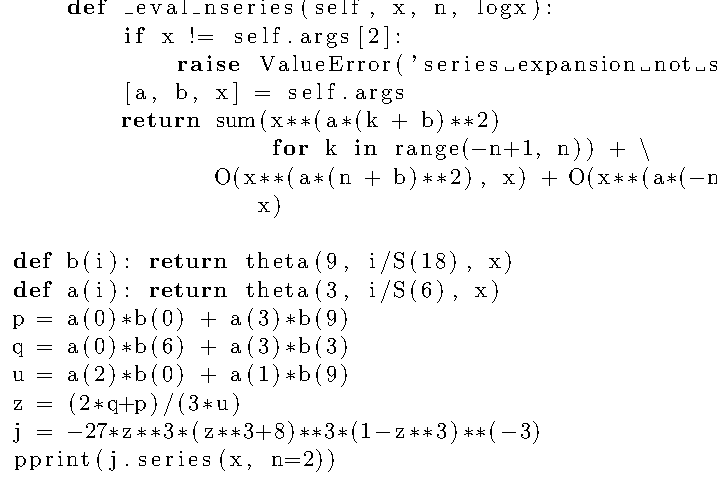
\includegraphics[width=0.60\textwidth]{figures/fig4.pdf}
  \caption{$x$ 空间：以 $x=-1,\,1,\,u,\,\infty$ 为分支点的双叶覆叠（亏格 1 的黎曼面）。两条割线分别连接
           $-1$ 与 $1$、$u$ 与 $\infty$；$a$-圈与 $b$-圈如图所示。原文仅标 “Figure 4”（原文 PDF 第 61 页），
           无说明性图注。}
  \label{fig:4}
\end{figure}

如此得到的 $x$ 空间正是一个亏格为 1 的黎曼面。这可以这样直观地看出：在环面上画一个圆 $c_1$，令其沿 $a$-圈环绕，再沿环面平移它得到圆 $c_2$（图 5(a)）。现在把圆 $c_1$ 与 $c_2$ 压扁成线段 $l_1$ 与 $l_2$
（图 5(b)）。这把环面分成沿这两条线段相接的两半。若把这两半都剪开，所得到的曲面就与上面描述的
$x$ 空间相同，其中 $l_1$ 与 $l_2$ 是两条分支割线，而无穷远点映为有限 $x$ 处的一点（图 5(c)）。

\begin{figure}[htbp]
  \centering
  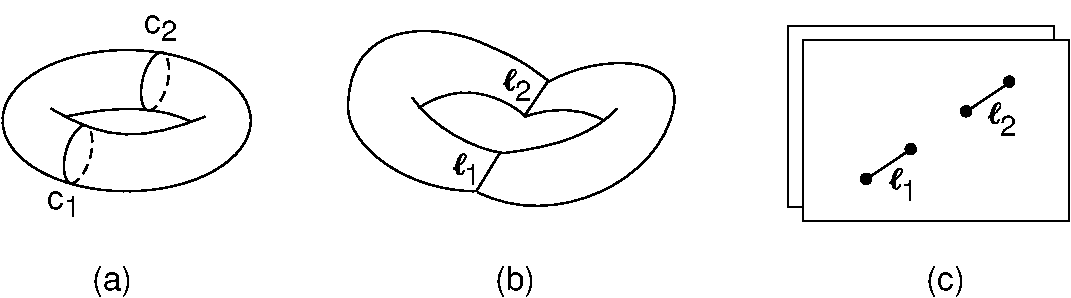
\includegraphics[width=0.95\textwidth]{figures/fig5.pdf}
  \caption{由环面理解 $x$ 空间。(a) 环面上的 $a$-圈 $c_1$ 与 $b$-圈 $c_2$；(b) 将 $c_1,c_2$ 压扁为线段
           $l_1,l_2$，环面被分成沿此二线段相接的两半；(c) 沿 $l_1,l_2$ 剪开两半后所得的双叶结构，即 $x$ 空间。
           原文仅标 “Figure 5”（原文 PDF 第 61 页），无说明性图注。}
  \label{fig:5}
\end{figure}

% [Tutor Note: 图 4、图 5（原文 PDF 第 61 页）。$y^2=(x-1)(x+1)(x-u)$ 对 $y$ 是二次的，故
%  $x$ 空间是 $\mathbf{C}\cup\{\infty\}$ 的双重覆叠，四个分支点 $-1,1,u,\infty$ 两两相连成两条割线；
%  割线的具体取法不唯一（这里取 $[-1,1]$ 与 $[u,\infty]$），不同取法只改变同调基的辛基底，不改变
%  物理。图 5 用环面说明：$c_1,c_2$ 压扁为 $l_1,l_2$ 后剪开，得到双叶结构；$x$ 平面上绕单条割线的
%  回路对应 $a$-圈，与两条割线都相交的回路对应 $b$-圈。]

由此清楚可见，$x$ 平面上绕两条割线之一走一圈的回路，对应环面的 $a$-圈；另一方面，与两条割线都
相交的回路（在我们的情形中，绕 $1$ 与 $u$），对应环面上的 $b$-圈。注意，当 $x$ 空间上两个分支点
重合时，曲线 $E_u$ 上的一个圈收缩为零，曲线变为奇异。例如在我们的情形中，若 $u=\infty$，
$a$-圈收缩为零；而 $u=1$ 时，这发生在 $b$-圈上。于是 $u$ 平面上的奇点正是族 $E_u$ 中某条曲线出现消失圈之处。

% [Tutor Note: 原文 PDF 第 62 页。奇点处消失圈与单值变换的对应是本节的核心：$u=\infty$ 时
%  $a$-圈收缩（对应 $M_\infty$），$u=1$ 时 $b$-圈收缩（对应 $M_1$）；由 $\mathbf{Z}_2$ 对称性
%  $u\to-u$，$u=-1$ 处同样是一个 $b$-圈收缩（对应 $M_{-1}$，但基底经 $a_D\to a-a_D$ 重排）。
%  这也解释了 $H/\Gamma(2)$ 为何恰有三个尖点——尖点即消失圈的位置。]

为确定 $a_D$ 与 $a$，在亏格为 1 的黎曼面 $E_u$ 上取两条独立的一维圈 $\gamma_1$ 与 $\gamma_2$，
并归一化使其相交数为 1：
$$
\gamma_1 \cdot \gamma_2 = 1\,.
$$
这些圈随 $u$ 连续变化，构成 $V_u=H^1(E_u,{\rm C})$ 这一 $E_u$ 的一阶同调群的局部基。一个圈可以与
一阶上同调群中的元素 $\lambda$ 配对：
$$
\gamma \rightarrow  \oint_{\gamma} \lambda\,.
$$
$\lambda$ 可看作亚纯 $(1,0)$-形式，定义在 $E_u$ 上，留数为零，模去恰当形式。留数为零保证该配对在
$\gamma$ 的连续形变下不变，即使形变越过 $\lambda$ 的极点。借助这一配对，我们也可把 $\lambda$
视为 $V_u$ 的元素。对 $E_u$ 上的 1-形式，可以取基底
$$
\lambda_{1} = \frac{dx}{y}\,, \qquad \lambda_{2} = \frac{xdx}{y}\,.
$$
不计标量倍数，$\lambda_1$ 是 $E_u$ 上唯一的全纯微分；若定义
$$
b_i=\oint_{\gamma_i}\lambda_1\,,\qquad{\rm for}\quad i = 1,2\,,
$$
则环面由参数
$$
\tau_u = b_1/b_2\,,\qquad {\rm with} \quad {\rm Im}(\tau_u) > 0\,. 
$$
刻画。考虑任意截面
$$
\lambda = a_1(u) \lambda_1 + a_2 (u) \lambda_2\,,
$$
（它是 $V_u$ 的截面），并暂时作如下等同：
$$
a_D=\oint_{\gamma_1}\lambda\,,\qquad a=\oint_{\gamma_2}\lambda\,.
$$
若 $\lambda$ 是留数为零的形式，则绕奇点一圈时 $a_D$ 与 $a$ 按正确的方式变换，这完全由
$\gamma_1$ 与 $\gamma_2$ 在 $SL(2,Z)$ 的某个子群下的变换决定（这一点在下面第 4.6 小节还会解释）。
另一方面，若 $\lambda$ 有一个留数非零的极点，则积分路径可能越过该极点，结果 $a_D$ 与 $a$ 可能
不再按纯粹的 $SL(2,Z)$ 变换。正如我们在前面某小节中已讨论的，在没有非零裸质量费米子的情形下，
这第二种可能性当然与 BPS 质量公式的对称性不一致。因此 $\lambda$ 不应有留数非零的极点（存在非零
裸质量费米子时情形不同，将在下一节末尾讨论）。上述对 $a_D$ 与 $a$ 的等同意味着
$$
\frac{da_D}{du}=\oint_{\gamma_1}\frac{d\lambda}{du}\,,\qquad
\frac{da}{du}=\oint_{\gamma_2}\frac{d\lambda}{du}\,.
$$
为固定 $\lambda$ 的任意性，我们利用条件 ${\rm Im}\tau > 0$，它正是 (\ref{tau-metric}) 所定义的
${\cal M}$ 上度规所要求的。首先设
$$
\frac{d\lambda}{du} = f(u) \lambda_{1} = f(u) \frac{dx}{y}\,.
$$
于是
$$
\frac{da_{D}}{du} = f(u)\,b_1\,,\qquad \frac{da}{du} = f(u)\,b_2\,,
$$
从而
$$
\tau = \frac{b_1}{b_2} = \tau_u\,. 
$$
由于 ${\rm Im}\,\tau_u > 0$，得到 ${\rm Im}\,\tau >0$。正如 Seiberg 与 Witten 所论证的，
逆命题也成立，因此 $d\lambda/du$ 不依赖于 $\lambda_2$。函数 $f(u)$ 由理论在 $u$ 平面奇点附近的
渐近行为固定，其值为 $f(u)=-\sqrt{2}/4\pi$。由此可得 $\lambda$ 为
$$
\lambda=\frac{\sqrt{2}}{2\pi}\;\frac{dx\sqrt{x-u}}{\sqrt{x^2-1}}=  
\frac{\sqrt{2}}{2\pi}\;\frac{dx y}{x^2-1}=\frac{\sqrt{2}}{2\pi}\;
\frac{dx}{y} (x-u) \,.
$$
为计算 $a$ 与 $a_D$，必须在 $E_u$ 上选取一组具体的一维圈基。我们把 $\gamma_2$ 等同于环面上的
$a$-圈，等价地，等同于一条绕点 $-1$ 与 $1$ 的曲线，这两个点取在 $x$ 平面上。可以把这条曲线形变到完全沿从 $-1$
到 $1$ 的割线来回。于是 $a(u)$ 由
\begin{equation}
a(u)=\frac{\sqrt{2}}{\pi}\,\int_{-1}^1\,\frac{dx\sqrt{x-u}}{\sqrt{x^2-1}}\,.
\label{au}
\end{equation}
给出。对 $\gamma_1$，取绕点 $1$ 与 $u$ 的曲线，得到
\begin{equation}
a_D(u)=\frac{\sqrt{2}}{\pi}\,\int_{1}^u\,\frac{dx\sqrt{x-u}}{\sqrt{x^2-1}}\,.
\label{adu}
\end{equation}
可以验证，在这样的圈选取下，$a$ 与 $a_D$ 在奇点附近具有所期望的行为 \cite{SW-I}。

% [Tutor Note: 原文 PDF 第 62 页。原文写 “first homology group $V_u=H^1(E_u,{\rm C})$”，严格说
%  $H^1$ 是上同调记号（同调应为 $H_1$）；因 $E_u$ 是紧致定向曲面，二者经 Poincaré 对偶同构，
%  后文按同调使用无碍，但引用时宜留意这一记号混用。留数为零的条件保证 $\oint_\gamma\lambda$
%  在 $\gamma$ 连续形变时不变（即使越过 $\lambda$ 的极点），这是 $\lambda$ 能作为 $V_u$ 元素并
%  与周期配对的前提。]

% [Tutor Note: 原文 PDF 第 63 页。由 $d\lambda/du=f(u)\,dx/y$ 与 $f(u)=-\sqrt2/4\pi$ 积分可得
%  $\lambda=\frac{\sqrt2}{2\pi}\frac{dx\sqrt{x-u}}{\sqrt{x^2-1}}$：因为
%  $\int du\,(x-u)^{-1/2}=-2\sqrt{x-u}$，负号与 $f$ 的负号相消，系数恰为 $\sqrt2/2\pi$。三个等号
%  用到 $y^2=(x^2-1)(x-u)$，即 $\frac{\sqrt{x-u}}{\sqrt{x^2-1}}=\frac{y}{x^2-1}=\frac{x-u}{y}$。
%  $\sqrt{x-u}$ 的分支约定与下面 $a_D$ 积分中出现的 $i$ 直接相关，不能随意选取。]

% [Tutor Note: 式 (\ref{au})、(\ref{adu})（原文编号 (107)、(108)，原文 PDF 第 63 页）。$\gamma_2$
%  沿 $[-1,1]$ 割线来回，故 $a(u)$ 的积分限为 $-1\to 1$；$\gamma_1$ 绕 $1$ 与 $u$，故积分限为
%  $1\to u$。两式的积分路径都取在相应割线的同一侧，上下限方向决定整体符号；若把 $\gamma_1$ 的
%  定向取反，$a_D$ 变号，继而 $M_1$、$M_{-1}$ 都会改变，务必与原文约定一致。原文在此引 \cite{SW-I}
%  验证了渐近行为。]

\noindent\underline{$a(u)$ 与 $a_D(u)$ 的显式表达式：}

容易求出 $a$ 与 $a_D$ 的显式表达式，其形式为完全椭圆积分 $E(k)$ 与 $K(k)$；所用的工具是
超几何函数 $F(\alpha,\beta,\gamma;z)$ 的积分表示 \cite{GR}。超几何函数由下式给出
\begin{eqnarray}
F(\alpha,\beta,\gamma;z)&=& \frac{\Gamma(\gamma)}{\Gamma(\beta)
\Gamma(\gamma-\beta)}\int_0^1\,dx\,x^{\beta-1} (1-x)^{\gamma-\beta-1}
(1-zx)^{-\alpha}\nonumber\\ 
&=& \frac{\Gamma(\gamma)}{\Gamma(\alpha)\Gamma(\beta)}\sum_{n\geq 0}
\frac{\Gamma(\alpha +n)\Gamma(\beta +n)}{\Gamma(\gamma +n)}\,
\frac{z^n}{n!}\,.\nonumber
\end{eqnarray}
将其与 (\ref{au}) 中 $a$ 的积分表示比较，容易看出
$$
a(u)=\sqrt{2(1+u)}\, F\left(-1/2, 1/2, 1; 2/(1+u)\right)\,.
$$
至于 $a_D$，先在 (\ref{adu}) 中作代换 $x=(u-1)t+1$。这给出
$$
a_D(u)=\frac{i}{\pi} (u-1)\int_0^1\,dt\,t^{-\frac{1}{2}}
(1-t)^{\frac{1}{2}} (1-\frac{1-u}{2} t)^{-\frac{1}{2}}\,. 
$$
将其与超几何函数的表达式比较，得到
$$
a_D(u)=\frac{i}{2} (u-1) F\left(1/2, 1/2, 2; (1-u)/2\right)\,.
$$

% [Tutor Note: 原文 PDF 第 64 页超几何函数的两种表示。积分表示前的 $\Gamma$ 因子是
%  $\Gamma(\gamma)/[\Gamma(\beta)\Gamma(\gamma-\beta)]$，而级数表示前是
%  $\Gamma(\gamma)/[\Gamma(\alpha)\Gamma(\beta)]$——两者并不相同，极易误抄成同一个；积分表示还要求
%  ${\rm Re}\,\gamma>{\rm Re}\,\beta>0$。另注意原文把 $F$ 的自变量写在分号之后
%  （$F(\alpha,\beta,\gamma;z)$），与某些文献的 $F(\alpha,\beta;\gamma;z)$ 记法只是标点差别。]

% [Tutor Note: 原文 PDF 第 64 页。在 $a_D$ 的积分 (\ref{adu}) 中作 $x=(u-1)t+1$，则
%  $x-u=(u-1)(t-1)$；在 $u>1$ 的割线一侧、$t\in[0,1]$ 上，
%  $\sqrt{x-u}=i\sqrt{u-1}\sqrt{1-t}$，同时
%  $\sqrt{x^2-1}=\sqrt{(u-1)t\,[(u-1)t+2]}$。整理后出现的 $i$、$(u-1)$ 以及
%  $(1-u)/2=-k'^2/k^2$ 中的负号，是这一段最易出错的地方，务必逐步核对。]

用超几何函数表示，完全椭圆积分为
\begin{eqnarray}
K(k) &=& \frac{\pi}{2}\, F\left(1/2, 1/2, 1; k^2\right)\,,\nonumber\\
E(k) &=& \frac{\pi}{2}\, F\left(-1/2, 1/2, 1; k^2\right)\,.\nonumber
\end{eqnarray}
进而定义 $k'^2=1-k^2$，并令
$$
E'(k)\equiv E(k')\,,\qquad K'(k) \equiv K(k')\,.
$$ 
现在利用恒等式
$$
c(1-z)F(a,b,c;z) - c F(a,b-1,c;z) + (c-a)z F(a,b,c+1;z)=0\,,
$$ 
取 $c=1, a=b=1/2$ 且 $z=(1-u)/2$，代入 $a_D$ 的表达式，得到
\begin{eqnarray}
a(u)   &=& \frac{4}{\pi k} E(k)\,,\nonumber\\
a_D(u) &=& \frac{4}{i\pi} E(i\frac{k'}{k}) + 
\frac{4i}{\pi k^2} K(i\frac{k'}{k})\,.\nonumber
\end{eqnarray}
这里 $k^2=2/(1+u)$，$(1-u)/2=-k'^2/k^2$。若注意到
$$
F(a, b, c; z)=(1-z)^{-a} F(a, c-b, c; z/(z-1))=
(1-z)^{-b} F(b, c-a, c; z/(z-1))\,.
$$
则这些表达式可以进一步简化。上式蕴含 $K(ik'/k)=kK(k')=kK'(k)$ 与
$E(ik'/k)=k^{-1}E(k')=k^{-1}E'(k)$，于是
\begin{eqnarray}
a(u)  &=& \frac{4}{\pi k}\, E(k)\,,\nonumber\\
a_D(u)&=& \frac{4}{\pi i}\,\frac{E'-K'}{k}\,.\nonumber
\end{eqnarray}
广义耦合 $\tau$ 可利用
\begin{eqnarray}
\frac{dE}{dk}&=&\frac{E-K}{k}\,,\quad 
\frac{dK}{dk}=\frac{1}{kk'^2}\,(E-k'^2 K)\,,\nonumber\\
\frac{dE'}{dk}&=&-\frac{k}{k'^2}\,(E'-K')\,,\quad 
\frac{dK'}{dk}=-\frac{1}{kk'^2}\,(E'-k^2 K')\,,\nonumber
\end{eqnarray}
算出，结果为
$$
\tau=\frac{\partial a_D}{\partial a}=\frac{da_D/dk}{da/dk}
=\frac{iK'}{K}\,.
$$

% [Tutor Note: 原文 PDF 第 64 页椭圆积分约定。这里 $K(k),E(k)$ 的宗量是模数 $k$，而不是参数
%  $m=k^2$：$K(k)=\frac{\pi}{2}F(1/2,1/2,1;k^2)$，$E(k)=\frac{\pi}{2}F(-1/2,1/2,1;k^2)$。原文只写
%  $E(k),K(k)$ 而未声明约定，引用文献数据时务必注意 $K(m)$ 与 $K(k)$ 相差一个 $k\to\sqrt m$
%  的代换；$k'^2=1-k^2$ 为补模。]

% [Tutor Note: 原文 PDF 第 65 页。$F(a,b,c;z)=(1-z)^{-a}F(a,c-b,c;z/(z-1))$ 是超几何函数的分式
%  线性变换，由此得 $K(ik'/k)=kK'(k)$、$E(ik'/k)=k^{-1}E'(k)$。注意 $|ik'/k|$ 一般不在 $[0,1)$
%  内，$K,E$ 需解析延拓；又 $E'$、$K'$ 是 $E(k')$、$K(k')$ 的简写，不是对 $k$ 的导数——原文的
%  撇号在这两节里有“补模”与“导数”两种含义，读到 $dE'/dk$ 时尤须分清。]

% [Tutor Note: 原文 PDF 第 65 页末。由 $a=\frac{4}{\pi k}E(k)$、
%  $a_D=\frac{4}{\pi i}\frac{E'-K'}{k}$ 对 $k$ 求导：
%  $\frac{da}{dk}=-\frac{4}{\pi}\frac{K}{k^2}$，
%  $\frac{da_D}{dk}=\frac{4}{\pi i}\frac{K'}{k^2}$（注意 $E'=E(k')$、$K'=K(k')$ 中 $k'^2=1-k^2$
%  也依赖 $k$，求导时不能漏掉 $dk'/dk=-k/k'$），二者相除才得 $\tau=iK'/K$。若漏掉补模对 $k$ 的
%  依赖，会得到相差一个 $k$ 因子的结果。]
